\chapter{Fondamenti di Sicurezza}

\section{Introduzione alla Sicurezza Informatica}

Per sicurezza informatica si intendono una serie di misure e controlli che assicurano la confidenzialità, l'integrità e la disponibilità delle risorse del sistema informativo, compresi l'hardware, il software, il firmware e le informazioni elaborate, memorizzate e trasmesse.

\subsection{La Triade CIA}

I tre obiettivi chiave al centro della sicurezza informatica, noti anche come \textbf{triade CIA}, sono fondamentali per qualsiasi architettura sicura:

\begin{defbox}[Confidentiality (Confidenzialità)]
Ossia preservare le autorizzazioni riguardo l'accesso e la divulgazione delle informazioni. Comprende:
\begin{itemize}
    \item \textbf{Confidenzialità dei dati:} assicura che le informazioni sensibili non siano rese disponibili a individui o processi non autorizzati.
    \item \textbf{Privacy:} assicura che gli individui controllino quali informazioni che li riguardano possano essere raccolte e conservate, nonché a chi possano essere divulgate.
\end{itemize}
\end{defbox}

\begin{defbox}[Integrity (Integrità)]
Ossia la protezione contro la modifica impropria o accidentale delle informazioni. Racchiude:
\begin{itemize}
    \item \textbf{Integrità dei dati:} assicura che le informazioni e i programmi siano modificati solo in un modo specificato e autorizzato.
    \item \textbf{Integrità del sistema:} assicura che un sistema esegua il suo compito prestabilito in modo ineccepibile, privo di manipolazioni esterne.
\end{itemize}
\end{defbox}

\begin{defbox}[Availability (Disponibilità)]
Assicura che i sistemi lavorino prontamente e che il servizio non sia negato agli utenti autorizzati quando ne hanno bisogno.
\end{defbox}

\subsection{Livelli di Impatto delle Violazioni}

La sicurezza informatica definisce tre livelli di impatto per valutare le conseguenze potenziali di una violazione, aiutando le organizzazioni a classificare il rischio:

\begin{itemize}
    \item \textbf{Basso:} La perdita potrebbe avere un effetto limitato (es. efficacia ridotta, piccoli disagi).
    \item \textbf{Moderato:} La perdita potrebbe avere un serio effetto negativo (es. operatività svolta con grandi difficoltà, danni finanziari misurabili).
    \item \textbf{Alto:} La perdita potrebbe avere un effetto negativo grave o catastrofico (es. impossibilità di svolgere le funzioni primarie, danni d'immagine irreparabili o pesanti sanzioni legali).
\end{itemize}


\section{Terminologia della Sicurezza}
Comprendere le relazioni tra gli elementi chiave della sicurezza è fondamentale. Le vulnerabilità rappresentano delle falle, mentre le minacce sono gli agenti che cercano di sfruttarle.

\begin{center}
\begin{tikzpicture}[
    node distance=1cm,
    box/.style={draw, rounded corners, text width=4.5cm, align=center, fill=gray!5, inner sep=1.5ex, font=\small},
    arrow/.style={->, >=stealth, thick}
]

\node[box] (asset) {\textbf{Asset}\\[1.5mm] La risorsa che si vuole difendere (sistema hardware, software o dati).};
\node[box, below=of asset] (vuln) {\textbf{Vulnerabilità}\\[1.5mm] Difetto o debolezza che espone il sistema al rischio di un attacco.};
\node[box, left=of vuln] (threat) {\textbf{Minaccia}\\[1.5mm] Evento o agente con il potenziale di causare danno sfruttando una vulnerabilità.};
\node[box, right=of vuln] (risk) {\textbf{Rischio}\\[1.5mm] Probabilità che la minaccia si realizzi $\times$ l'Impatto conseguente.};
\node[box, below=of risk] (counter) {\textbf{Contromisura}\\[1.5mm] Azione o dispositivo che riduce minaccia, vulnerabilità o impatto.};
\node[box, below=of threat] (attack) {\textbf{Attacco}\\[1.5mm] Attività malevola intenzionale per raccogliere, interrompere o distruggere.};

\draw[arrow] (threat) -- node[above, font=\footnotesize] {sfrutta} (vuln);
\draw[arrow] (threat) -- node[left, font=\footnotesize] {concreta} (attack);
\draw[arrow] (attack) -- node[below, font=\footnotesize] {mira a} (vuln);
\draw[arrow] (vuln) -- node[left, font=\footnotesize] {espone} (asset);
\draw[arrow] (vuln) -- node[above, font=\footnotesize] {genera} (risk);
\draw[arrow] (risk) -- node[right, font=\footnotesize] {danneggia} (asset);
\draw[arrow] (counter) -- node[right, font=\footnotesize] {mitiga} (risk);
\draw[arrow] (counter) -| node[near start, below, font=\footnotesize] {riduce} (vuln);

\end{tikzpicture}
\end{center}

\subsection{Modelli di Controllo degli Accessi}
\begin{defbox}[Modelli di Accesso: RBAC e ABAC]
\begin{itemize}
    \item \textbf{RBAC (Role-Based Access Control)}: Il controllo è basato sui \textit{ruoli} (es. amministratore, utente base, revisore) a cui gli utenti vengono assegnati in base alle loro mansioni. Semplifica enormemente la gestione dei permessi nelle grandi organizzazioni, poiché i diritti sono associati al ruolo e non al singolo utente.
    \item \textbf{ABAC (Attribute-Based Access Control)}: Modello molto più granulare e dinamico. I permessi vengono valutati in tempo reale in base agli \textit{attributi} del soggetto (es. dipartimento), dell'oggetto (es. livello di classificazione) e dell'ambiente (es. orario di accesso, posizione geografica, tipo di rete).
\end{itemize}
\end{defbox}

\section{Tipologie di Attacco e di Minacce}

\subsection{Classificazione degli Attacchi}

Gli attacchi possono essere classificati secondo diverse dimensioni, principalmente in base all'interazione con il sistema:

\begin{warnbox}[Attacchi: Passivi vs Attivi]
\begin{description}
    \item[Attacco passivo] Consiste nel tentativo di apprendere o utilizzare informazioni dal sistema senza alterarne le risorse o il funzionamento (es. intercettazione del traffico di rete, sniffing). L'obiettivo principale della difesa contro di essi è la \textbf{prevenzione}, tipicamente tramite la cifratura, in quanto sono difficili da rilevare.
    \item[Attacco attivo] Comporta il tentativo esplicito di alterare le risorse del sistema o di influenzarne pesantemente il funzionamento (es. iniezione di codice, modifica di file, denial of service). L'obiettivo principale della difesa in questo caso è la \textbf{rilevazione} tempestiva e la pronta risposta.
\end{description}
\end{warnbox}

Un'altra classificazione importante si basa sull'origine dell'attacco:
\begin{itemize}
    \item \textbf{Attacco interno (Insider Threat):} Effettuato da un utente autorizzato ad accedere al sistema, ma che abusa dei propri privilegi per fini illeciti. Spesso è il più difficile da fermare poiché l'attaccante è già all'interno del perimetro difensivo.
    \item \textbf{Attacco esterno:} Effettuato da un \textit{outsider}, ossia un soggetto non autorizzato che tenta di forzare le difese permetrali dall'esterno.
\end{itemize}

\subsection{Le Minacce Specifiche}

Le minacce informatiche possono essere raggruppate in quattro categorie fondamentali a seconda dell'obiettivo e dell'effetto che producono sulle risorse del sistema.

\begin{warnbox}[1. Divulgazione Non Autorizzata]
La divulgazione non autorizzata (\textit{unauthorized disclosure}) è una minaccia diretta alla confidenzialità. I seguenti attacchi possono causarla:
\begin{itemize}
    \item \textbf{Esposizione (exposure):} Può essere intenzionale o risultato di un errore umano/software, traducendosi nella conoscenza non autorizzata di dati sensibili.
    \item \textbf{Intercettazione (interception):} Ricezione di una copia di informazioni in transito destinate originariamente a un altro dispositivo (es. man-in-the-middle).
    \item \textbf{Inferenza (inference):} Nota anche come analisi del traffico; l'avversario ottiene informazioni preziose semplicemente osservando il pattern del traffico o incrociando dati apparentemente innocui.
    \item \textbf{Intrusione (intrusion):} Ottenimento di un accesso illegittimo a dati sensibili eludendo le protezioni del sistema.
\end{itemize}
\end{warnbox}

\begin{warnbox}[2. Inganno]
L'inganno (\textit{deception}) è una minaccia che compromette l'integrità del sistema o dei dati:
\begin{itemize}
    \item \textbf{Mascheramento (masquerade):} Tentativo di un utente non autorizzato di accedere al sistema fingendosi un utente autorizzato o un'entità legittima.
    \item \textbf{Falsificazione (falsification):} Alterazione fraudolenta o sostituzione di dati validi con dati falsi o manipolati.
    \item \textbf{Ripudio (repudiation):} Situazione in cui un utente nega falsamente di aver compiuto un'azione, come l'invio o la ricezione di un messaggio.
\end{itemize}
\end{warnbox}

\begin{warnbox}[3. Interruzione]
L'interruzione (\textit{disruption}) mira ad abbattere la disponibilità o l'integrità del sistema:
\begin{itemize}
    \item \textbf{Interdizione (incapacitation):} Attacco brutale alla disponibilità (es. danneggiamento fisico dell'hardware o disattivazione dei servizi tramite malware distruttivo).
    \item \textbf{Corruzione (corruption):} Attacco all'integrità in cui le risorse o i servizi vengono manipolati per funzionare in modo non previsto o errato.
    \item \textbf{Ostruzione (obstruction):} Interferenza con le comunicazioni, che avviene disabilitando i collegamenti di rete o sommergendo il sistema di traffico anomalo.
\end{itemize}
\end{warnbox}

\begin{warnbox}[4. Usurpazione]
L'usurpazione (\textit{usurpation}) è una grave minaccia all'integrità del sistema stesso:
\begin{itemize}
    \item \textbf{Appropriazione indebita (misappropriation):} Furto o dirottamento di un servizio, come ad esempio l'uso non autorizzato di un server aziendale come piattaforma per lanciare attacchi DDoS (Distributed Denial of Service) verso terzi o per minare criptovalute.
    \item \textbf{Uso improprio (misuse):} Disabilitazione o aggiramento attivo delle funzioni di sicurezza da parte di chi sfrutta falle o privilegi non dovuti, assumendo il controllo delle operazioni protette.
\end{itemize}
\end{warnbox}

\section{Valutazione delle Minacce}

\subsection{Superfici di Attacco}
Una \textbf{superficie di attacco} rappresenta l'insieme totale di tutte le vulnerabilità raggiungibili e teoricamente sfruttabili all'interno di un sistema. Si divide comunemente in tre macro-aree:
\begin{itemize}
    \item \textbf{Superficie di Rete}: Include porte aperte, protocolli di rete deboli, interfacce web, VPN e punti di accesso wireless.
    \item \textbf{Superficie Software}: Comprende le vulnerabilità insite nel codice delle applicazioni, nel sistema operativo e nelle librerie di terze parti utilizzate.
    \item \textbf{Superficie Umana}: Rappresenta le vulnerabilità legate alle persone, tra cui la suscettibilità ad attacchi di ingegneria sociale (es. phishing) o la propensione a commettere errori operativi.
\end{itemize}

\begin{notebox}[Analisi della Superficie]
L'\textbf{analisi della superficie di attacco} è una tecnica cruciale per valutare concretamente l'esposizione alle minacce. L'obiettivo ultimo di un'architettura sicura è quello di \textit{ridurre tale superficie} il più possibile, chiudendo le porte inutilizzate e minimizzando i servizi in esecuzione, per rendere esponenzialmente più difficile il compito dell'avversario.
\end{notebox}

Il seguente grafico mostra il rapporto tra la dimensione e la profondità della superficie di attacco e il relativo rischio di sicurezza.

\begin{center}
    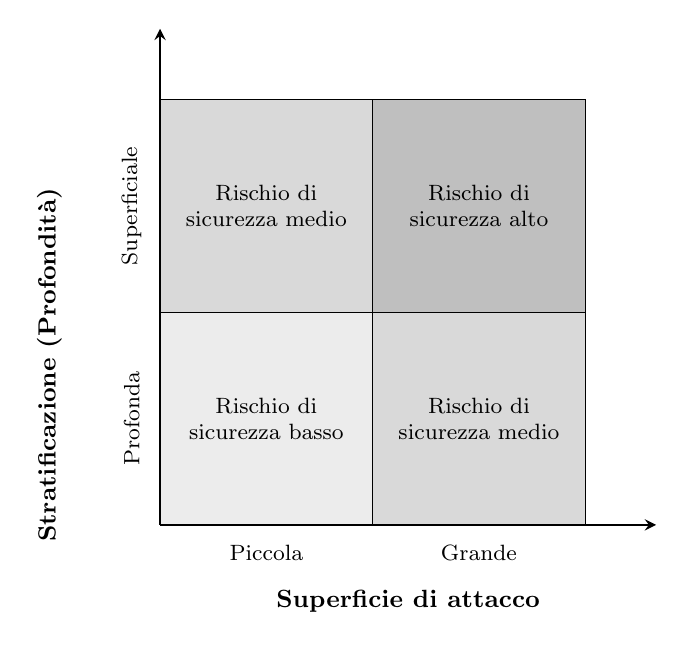
\begin{tikzpicture}[>=stealth, font=\footnotesize, scale=0.9]

    % Definizione dei colori (sfumature di grigio/azzurro)
    \colorlet{lightgray}{gray!15}
    \colorlet{mediumgray}{gray!30}
    \colorlet{darkgray}{gray!50}

    % Quadranti (Riempimento e Bordi)
    % In basso a sinistra
    \fill[lightgray] (0,0) rectangle (3,3);
    \draw (0,0) rectangle (3,3) node[midway, align=center] {Rischio di\\sicurezza basso};
    
    % In alto a sinistra
    \fill[mediumgray] (0,3) rectangle (3,6);
    \draw (0,3) rectangle (3,6) node[midway, align=center] {Rischio di\\sicurezza medio};
    
    % In basso a destra
    \fill[mediumgray] (3,0) rectangle (6,3);
    \draw (3,0) rectangle (6,3) node[midway, align=center] {Rischio di\\sicurezza medio};
    
    % In alto a destra
    \fill[darkgray] (3,3) rectangle (6,6);
    \draw (3,3) rectangle (6,6) node[midway, align=center] {Rischio di\\sicurezza alto};

    % Assi con frecce
    \draw[->, thick] (0,0) -- (7,0) node[below=20pt, pos=0.5, font=\small\bfseries] {Superficie di attacco};
    \draw[->, thick] (0,0) -- (0,7) node[left=40pt, pos=0.7, rotate=90, font=\small\bfseries] {Stratificazione (Profondità)};

    % Etichette Assi (Piccola/Grande e Profonda/Superficiale)
    \node at (1.5, -0.4) {Piccola};
    \node at (4.5, -0.4) {Grande};
    
    \node[rotate=90] at (-0.4, 1.5) {Profonda};
    \node[rotate=90] at (-0.4, 4.5) {Superficiale};

\end{tikzpicture}
\end{center}

\section{Minacce alle Risorse del Sistema}

Le minacce possono colpire le diverse categorie di risorse di un sistema informatico, violando uno o più princìpi della triade CIA in modi specifici:

\begin{table}[h!]
\centering
\renewcommand{\arraystretch}{1.5}
\begin{tabularx}{\textwidth}{|>{\bfseries}l|X|X|X|}
\hline
\rowcolor{gray!20} & \textbf{Disponibilità} & \textbf{Confidenzialità} & \textbf{Integrità} \\ \hline
Hardware & L'attrezzatura (server, router) viene rubata o disabilitata, impedendo l'erogazione del servizio. & Sottrazione di dispositivi (es. USB) non cifrati, esponendo i dati contenuti. & Dispositivi alterati fisicamente (es. keylogger hardware) o danneggiati. \\ \hline
Software & Cancellati o corrotti file eseguibili essenziali, bloccando l'avvio delle applicazioni. & Copia non autorizzata di software proprietario (furto di proprietà intellettuale). & Programma modificato per fallire o eseguire operazioni malevole nascoste (es. Trojan). \\ \hline
Dati & File essenziali cancellati o cifrati da ransomware, bloccando l'operatività. & Lettura, esfiltrazione non autorizzata o inferenza statistica sui dati esposti. & Modifica fraudolenta dei record in un database o iniezione di nuovi dati illeciti. \\ \hline
\end{tabularx}
\caption{Minacce alle risorse del sistema raggruppate in base alla triade CIA.}
\end{table}
